\chapter{Conclding Remarks} \label{ch:concldingRemarks}
In this final chapter, first of all, the results obtained with the test demo of the project developed during the course are presented, then an analysis is made in relation to the objectives proposed by the thesis, evaluating what has been achieved and the future work that can be related to the project.

This chapter aims to be a conclusion for the thesis work done, both from the descriptive side by providing a summary of the work done, and from the practical side of project development, but also with the purpose of providing open options for furthering the project. The \gls{ac:sdv} technologies are very young and there are many development ideas. In addition, as an open project with the objective of creating a standard for the entire automotive industry, there are many opportunities for collaboration.

Let's start the description with the conclusions gathered with the final test demo of the project on \textit{Raspberry Pi}.

\section{Test and Validation on Raspberry Pi}
To create the test demo, a \textit{Raspberry Pi 4} board was used, with an architecture based on \textit{Cortex-A72}, a processor from the \textit{Arm} family. This device was found to be the best solution for simulating a modern automotive \gls{ac:tcu} physical system.

First of all, it was necessary to instantiate the cloud stacks of \gls{ac:aws} services so that the supporting cloud structure was operational and ready to interact with the board. Once the necessary certificates for communication with the cloud platform had been obtained, it was possible to insert the communication scripts on the \textit{Raspberry Pi}.

Once the script was started, the communication was successful and the generated data arrived at the cloud server ready to be analyzed, as shown in the image \ref{fig:RaspberryPiDemo}. The only difference compared to the simulations performed on a local virtual machine was the time it took to receive the data. In particular, in the case of the \textit{Raspberry Pi}, there was a delay in sending data, although it was almost imperceptible and acceptable for the purposes of the test.
\begin{figure}[h]  % 'h' significa che la figura viene posizionata qui
    \centering
    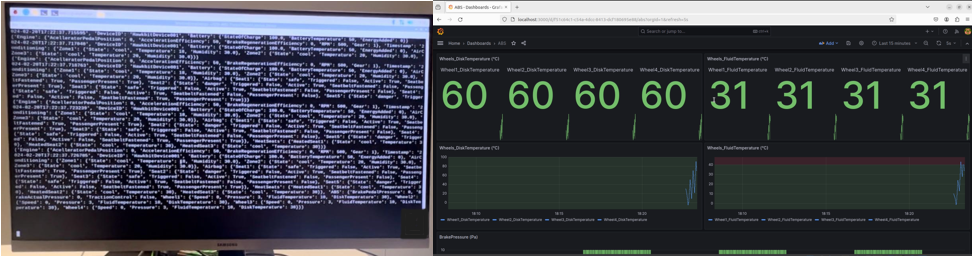
\includegraphics[width=0.9\textwidth]{images/RaspberryPiDemo.png}  % Sostituisci 'nome_immagine' con il nome del tuo file immagine e l'estensione
    \caption{Comunication between the \textit{Raspberry Pi} board and the \textit{Grafana} server via the AWS cloud services}
    \label{fig:RaspberryPiDemo}
\end{figure}

At this point, it was possible to start the update using the \textit{AWS CodePipeline} service. In particular, once the update process was started on the pipeline, it was able to correctly contact the \textit{Hawkbit} server where the \gls{ac:tcu} simulator was already present to start the update. 
Also in this case, it was necessary to wait a few more seconds for the update to be received on the device, but once this happened, the \textit{Raspberry Pi} was able to interrupt the flow, receive the update, and restart the system with the updated features. 
As shown in the figure \ref{fig:RaspberryPiDemoUpdate}, the update was also detected by the data analysis server. Specifically, both the \textit{Python} updates, which showed a drastic change in the data sent, and the update compiled in \textit{C}, which caused an interruption in the sending of data, as expected by the update itself were launched on the demo board.

The presentation of test demos on the \textit{Raspberry Pi} board was useful from several points of view and showed the following characteristics
\begin{itemize}
    \item The ability of the system to communicate through the \gls{ac:mqtt} protocol across different connection networks.
    \item The capability of the software simulator to be used on different platforms, including \textit{Arm}.
    \item The flexibility to adapt the cloud infrastructure to different conditions, whether it is a virtual machine or a physical board.
    \item Correct implementation of the pipeline capable of computing update projects written in compiled languages.
\end{itemize}
\begin{figure}[h]  % 'h' significa che la figura viene posizionata qui
    \centering
    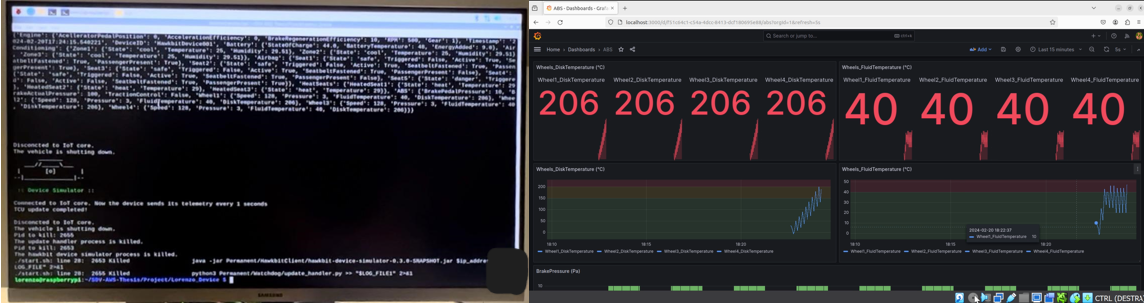
\includegraphics[width=0.9\textwidth]{images/RaspberryPiDemoUpdate.png}  % Sostituisci 'nome_immagine' con il nome del tuo file immagine e l'estensione
    \caption{Update to the \textit{Raspberry Pi} board and \textit{Grafana} data after the update}
    \label{fig:RaspberryPiDemoUpdate}
\end{figure}

\section{Contribution Recaps}
The aim of the thesis was to show the innovations introduced by the \gls{ac:sdv} technology, which is capable of completely revolutionizing the automotive industry. This result was achieved thanks to the support of the partner company, which provided the necessary resources to study, understand and analyze the cloud services offered by \gls{ac:aws}, but also to put them into practice in the implementation of the project, which included technologies currently used by several companies in the automotive sector.

The \gls{ac:sdv} represents a true innovation in the automotive field, as it would allow the industry to move forward in creating more efficient and safer vehicles. In addition, it would open the door to a different and innovative development and production method that could significantly reduce production costs and times, thereby reducing the waste of necessary resources.

The thesis has certainly achieved its objectives, but let's now evaluate whether the objectives of the project, which was created to give a practical demonstration of the cooperation between the various elements involved in the \gls{ac:sdv}, have been achieved.

\subsection{Are the PoC goals being met?}
One of the main objectives of the proof of concept was to demonstrate how the cloud infrastructure composed of services provided by \gls{ac:aws} could support the development of the \gls{ac:sdv} by using its resources. Certainly, this objective was fully achieved with the use of more than one pipeline responsible for managing updates. In particular, both the updates in \textit{Python} language, easily portable from one platform to another, and the updates in compiled languages, more targeted and specific to each platform, but also more optimized and closer to the real use case, were successfully carried out.

Another important goal of the work was to be able to bring together different technologies to support the creation of the infrastructure. Specifically, the project succeeded in making \gls{ac:aws} cloud services work with the \textit{Hawkbit} system (already under development in several automotive companies) for managing the deployment of updates, and with \textit{Grafana} services for data analysis. Achieving this goal made it possible to make the most of the technologies offered at the lowest possible cost to the company, obtaining a true ecosystem that is as open as possible.

As a final goal of the project, we can identify the need to introduce general purpose systems to support the development of the \gls{ac:sdv}. Also in this case, as seen before, the demo on the \textit{Raspberry Pi} board showed that it can interact masterfully with different general purpose platforms and make the best use of the available resources.

In conclusion, the results obtained at the beginning of the implementation can be considered as achieved. However, it is important to emphasize that the \gls{ac:poc} was a demonstration example, still in its early stages as far as actual production is concerned. The remaining points, deliberately left open due to limited resources, will be addressed below.

\section{Future Works}
Now the open aspects for the future development of the project are analyzed. In consideration of the nature of the work, some aspects were deliberately neglected in order to achieve a complete and functional result. If there had been an ambition to create a fully functional product on a real vehicle ready for use, not even a small part of the project could have been achieved with the available resources. Now let's talk about future work.

\subsection{Transform the PoC in a product}
To transform the proof of concept into a real product, usable in an automotive system capable of producing vehicles, it is necessary to cover three different steps: interfacing with a real vehicle to study the operational dynamics of a real \gls{ac:tcu} with all the subsystems that compose it, delving into the detailed analysis of the free software used such as \textit{Hawkbit}, and managing additional elements of the vehicle such as machine learning or cockpit applications. A brief overview of each of these future works is given below.
\begin{enumerate}
    \item Making the system usable with a real vehicle is essential to creating a market-ready commercial product. A real vehicle is made up of dozens, if not hundreds, of subsystems interconnected at various levels, and the management of all the data produced may be slightly different from what is seen in the \gls{ac:poc}. The telemetry systems of real vehicles contain security systems that prevent direct connection to each individual subsystem, for example through firewalls; this is another aspect to consider when building a real product.
    \item Another fundamental aspect for the creation of a concrete product is the in-depth analysis of the operational dynamics of the free software used in the development of the infrastructure. In particular, with regard to the \textit{Hawkbit} server, in the \gls{ac:poc}, after a not too detailed analysis of the various components, it was decided to use a pre-built \textit{Docker} image. This made it easier to manage the elements, since everything was ready, but limited the freedom of customization. To fully exploit the potential of these technologies, it will be essential to fully customize the software used, as happens in real companies.
    \item Last, but not least, is the adaptability of the \gls{ac:sdv} system to additional elements of the vehicle, such as machine learning systems for decision making or cockpit systems. For the \gls{ac:poc} to become a usable product in reality, it is essential that it is fully integrated into the vehicle. Therefore, it is inconceivable that there are systems in the vehicle itself that do not interface with the \gls{ac:sdv} system, especially if they are other systems strictly related to \gls{ac:it}, such as those mentioned above.  
\end{enumerate}

In conclusion, the full integration of the \gls{ac:poc} with a real vehicle represents an essential phase in the development of the technologies covered in the thesis. This would allow vehicles to be transformed into fully upgradeable devices, thus contributing to the improvement of efficiency and safety, fundamental elements in the automotive sector.